% Author: Izaak Neutelings (October 2020)
% Inspiration: https://tex.stackexchange.com/questions/25531/adding-underbrace-in-tikz
\documentclass[border=3pt,tikz]{standalone}
\usepackage{physics}
\usepackage{siunitx}
\usepackage{ifthen}
\usepackage{tikz}
%\usepackage[outline]{contour} % glow around text
\usetikzlibrary{calc}
\usetikzlibrary{angles,quotes} % for pic
\usetikzlibrary{patterns}
\tikzset{>=latex} % for LaTeX arrow head
%\contourlength{1.4pt}

\colorlet{xcol}{blue!70!black}
\colorlet{vcol}{green!70!black}
\colorlet{myred}{red!65!black}
\colorlet{acol}{red!50!blue!80!black!80}
\tikzstyle{ground}=[preaction={fill,top color=black!10,bottom color=black!5,shading angle=20},
                    fill,pattern=north east lines,draw=none,minimum width=0.3,minimum height=0.6]
\tikzstyle{metal}=[fill,top color=black!40,bottom color=black!20,shading angle=10]
\tikzstyle{mass}=[line width=0.6,red!30!black,fill=red!40!black!10,rounded corners=1,
                  top color=red!40!black!20,bottom color=red!40!black!10,shading angle=20]
\tikzstyle{rope}=[brown!70!black,very thick,line cap=round]
\def\rope#1{ \draw[black,line width=1.5] #1; \draw[rope] #1; }

% FORCES SWITCH
\tikzstyle{force}=[->,myred,very thick,line cap=round]
\tikzstyle{Fproj}=[force,myred!40]
\newcommand{\vbF}{\vb{F}}
\newcommand{\vbT}{\vb{T}}

\begin{document}
% CIRCULAR MOTION - force balance
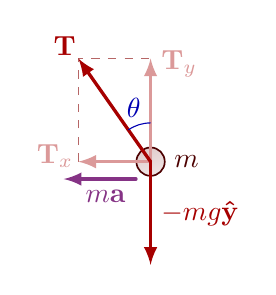
\begin{tikzpicture}
    \def\ang{35}   % angle
    \def\F{1.6}    % force size
    \def\r{0.18}   % ball radius
    \coordinate (O) at (0,0);
    \coordinate (F) at (90+\ang:\F);
    \coordinate (Fy) at (90:{\F*cos(\ang)});
    \coordinate (Fx) at (180:{\F*sin(\ang)});
    \draw[thin,mass] (O) circle (\r) node[right=5] {$m$};
    \draw[dashed,myred!80!black!60] (Fx) -- (F) -- (Fy);
    \draw[Fproj] (O) -- (Fy) node[below=2,right=0] {$\vbT_y$};
    \draw[Fproj] (O) -- (Fx) node[above=2,left=-2] {$\vbT_x$};
    \draw[force] (O) -- (F) node[above left=-3] {$\vbT$};
    \draw[force] (O) --++ (-90:{\F*cos(\ang)}) node[midway,right=0] {$-mg\vu{y}$};
    \draw[force,acol] (O)++(-130:1.6*\r) --++ (Fx) node[midway,right=2,below=0] {$m\vb{a}$};
    \draw pic["$\theta$",xcol,draw=xcol,angle radius=14,angle eccentricity=1.45] {angle=Fy--O--F};
\end{tikzpicture}

\end{document}